\documentclass[sigconf]{acmart}

\usepackage{hyperref}

\usepackage{endfloat}
\renewcommand{\efloatseparator}{\mbox{}} % no new page between figures

\usepackage{booktabs} % For formal tables

\settopmatter{printacmref=false} % Removes citation information below abstract
\renewcommand\footnotetextcopyrightpermission[1]{} % removes footnote with conference information in first column
\pagestyle{plain} % removes running headers

\begin{document}
\title{Big Data and Analytics in Block Chain}


\author{Ashok Kuppuraj}
\orcid{1234-5678-9012}
\affiliation{%
  \institution{Indiana University}
  \streetaddress{}
  \city{Bloomington} 
  \state{Indiana} 
  \postcode{43017-6221}
}
\email{akuppura@iu.edu}


% The default list of authors is too long for headers}
\renewcommand{\shortauthors}{G. v. Laszewski}


\begin{abstract}
This paper describes on how Big data and its technologies helps in augmenting or improving the current Block chain technology and overcome  the problems around it .
\end{abstract}

\keywords{Big Data, Block Chain i523}


\maketitle

\section{Introduction}
The objective is to concur the abilities of the two broad topics in the current technology world, the Big Data and Block Chain. Block chain and Big data both are still a evolving technologies, which gives us enough opportunity to explore and invent new concepts for its own good. As these are still evolving, we can leverage ones solution on the other.  To leverage each ones problems and solutions, we must first identify the similarities in  two frameworks and how these similarities are related and what solution we are going to adopt. 

 \cite{editor00}.

\section{What is Big Data}
Big data can be described as any type of data with large volume, velocity and variety \cite{Bigdataintro}. The history of Big data starts the moment we started using the computer back in 90s, however we choose not to use all the generated data due to constraints in the processing system, later we understood we are missing lots of information useful to the business due to these constraints, and we started leveraging Data warehouse to processes the data in Batch after the data generation . At certain point of time even the data warehouse systems are not capable to handle the volume and velocity of data we are generating. This exponential growth in the data generation due to wide adoption of computers by humans in the form of Mobile, PCs and introduction of IoT sensors, resulted in the term called "Big Data" \cite{article2}

\section{Block Chain}
Blockchain can defined as the decentralized, public ledger persisted in a connected set of immutable Blocks. The core idea is to perform any set of transaction without a governing third party avoiding Double spending by Distributed consensus. A transaction happens with an entity called tokens, Tokens are the actual digital asset of a blockchain. The implementation begins with an entity initiate the transaction, the initiated transaction request from A to B is broadcasted with Gossip protocol to most of the nodes, the transaction is validated by miners with the ledger available with them, validation includes checking digital signatures and the previous input to that entity (i.e current withholding), upon successful validation, it will be added in a block, a grouping of transaction records with previous address as the current block, which in turn has to be accepted by most of the nodes.Once most of the nodes accepts the transaction  will be added to the ledger confirming the transaction.

\section{Bigdata vs BlockChain}
As far as data is concerned, both Big data technologies and Blockchain goes in parallel.Both involves processing high volume of data at volume, velocity and variety which is the basic evaluation factor for defining big data, in the below sections, we will discuss how these three V's corresponds to Block Chain in a future perspective with an example data from Bitcoin, one of the front runners in implementing Blockchain technologies.

\subsection{Data Volume}
Though the data volume share of block chain is considerably low comparable with current Big data average, the volume it generates in a overall network perspective in terms of network I/O, logs, transaction data, it fits well with the terms of `big data. For example, consider the transaction growth of Bitcoin \cite{bitcointrans}, the volume of transaction was averaging 5K in 2011, whereas in 2017 the average is 200K with an increase of 400 percent over 5 years and the volume is likely to grow in an exponential scale with the global acceptance of Block chain technologies. 

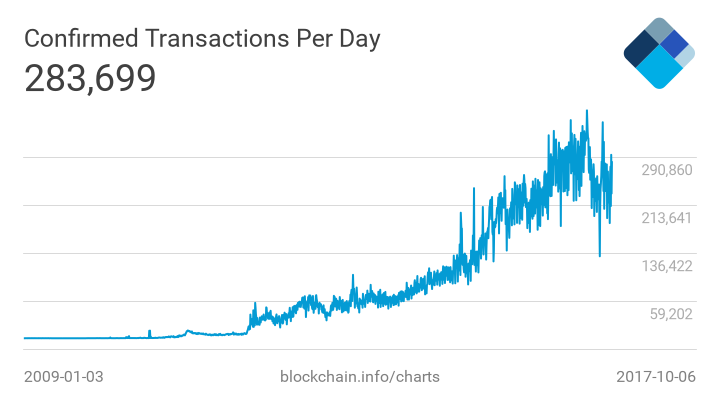
\includegraphics[scale=0.35]{paper1/images/bitcoin-trans.png}
\subsection{Data velocity}
In data terms, even 10 MB of data is considered huge when its getting generated with in a span of minute, hence we must consider the velocity as an important metric in analyzing the data, here in Bock chain, though the transactions are not of high volume, but other non=token transactions like Gossip calls, smart contract transfers, block transfers, acceptance protocol were happening every seconds, which in turns generate huge amount of data within 10 minutes of these interval with respect to Bitcoin.

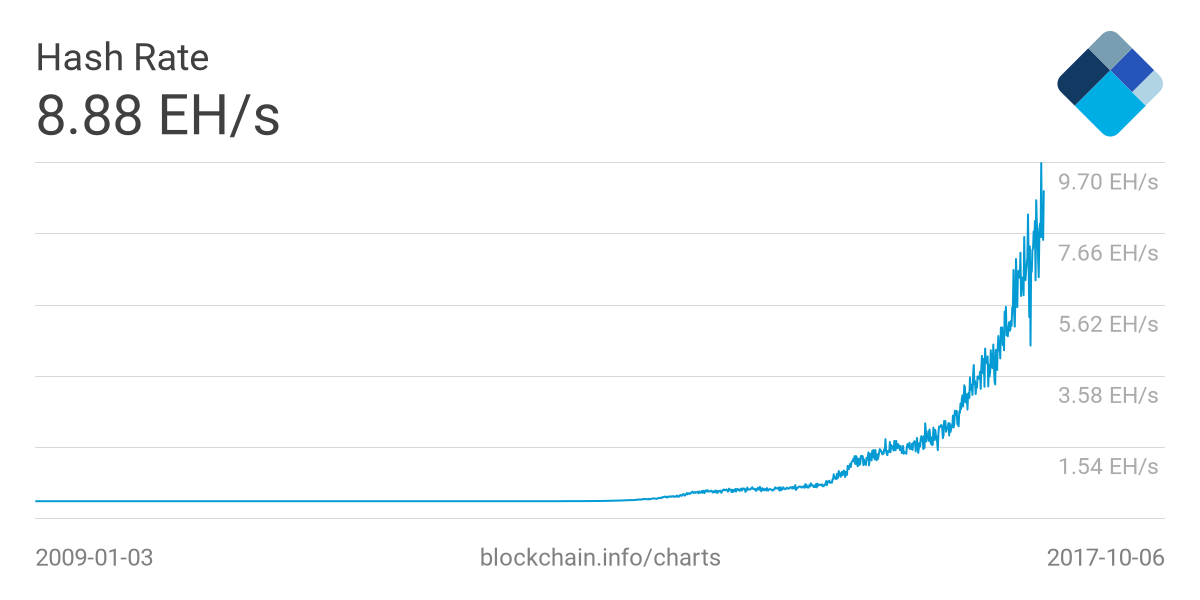
\includegraphics[scale=0.2]{paper1/images/hash-rate.png}
The snippet descriptes the number of hashes resolved per second, in Bitcoin's network \cite{hastratepersec}.

\subsection{Data Variety}
In a wide perspective, Blockchain deals with multiple varieties of structured data like Token data, Smart contracts, consensus data, logging data and unstructured data like videos \cite{livepeer-BC}, audio depending upon the use-case of the Blockchain. And the popularity it has now and based on the current growth trend in the acceptance of decentralization, Blockchain technology will tend to generate more data in wide range of varieties.


\section{Implementation - Big data technologies in Blockchain}
Before we start on the implementation of Big data technologies, its required to identify the problems Blockchain faces now in scope with Big data's solutions, one of the main problems are Slow transactions, complex analytical calculation through visualization. Though we have other problems, we consider the above two as the most important to enhance the success rate of this technology.
For example, consider Bitcoin, the overall transaction timing is very less in-terms of inter bank transaction however for the end user it takes minimum of 20 mins to complete a transaction whereas in Visa for instance, it can perform upto 1700 transaction per seconds.

\subsection{Transaction processing}
To deal with improving the transaction speed of a peer-to-peer network, first it is required to streamline the asynchronous process of gossip protocols, handshake between peers to increase the transaction processing speed and also by removing the block size limits\cite{Optimize} we can increase the frequency of the block building, this can be achieved with the help of Big data queuing utilities like Apache Kafka by creating individual topics for each set of Broadcasting, Block Acknowledgement, and consensus sharing between the peers,   and second is to increase the Hash processing capacity by horizontal scaling with the help of Big data technologies like Apache Spark or Apache Flink. By using these open source tools for hash processing, its not required to invest on high value GPU's to process data.

For example,kafka can handle upto 200,000 messages/second (220MB/second)\cite{kafka_performance}, which is way more than the any other existing banking can provide.



\subsection{Visualization}
The current visualization options available with blockchain is based on the shared ledger available in the network, to fetch a real time reporting or visualizing the happenings in the network, one must have to take part in the network and share all the interactions and the ledger details for any sort of analytical needs, as discussed in the previous section, if we start using Kafka for other peer-to-peer interactions via topics, we can seamlessly provide real-time reporting users.

\subsection{Smart-BlockChain}
The next big leap in the Blockchain would be implementation of Machine learning in the Block chain. The current stage of block chain don't give any machine learning modules or algorithm attached built along with. By including the machine learning modules in the blockchain network, Blockchain can be made smart by predicting malicious activities, optimized transactions, dependencies evaluation.


\section{Conclusion}
Although Blockchain can be considered a DB provides lots of solutions for the Real life problems, it would be nearly impossible without its implementations leaning towards Big data's solutions. Some of the 



\begin{acks}

  The authors would like to thank Dr. Gregor von Laszewski for his
  support and suggestions to write this paper.

\end{acks}

\bibliographystyle{ACM-Reference-Format}
\bibliography{report} 

\end{document}

